\documentclass{ieeeojies}
\linespread{1.125}
\usepackage{cite}
\usepackage{amsmath,amssymb,amsfonts}
\usepackage{algorithmic}
\usepackage{graphicx}
\usepackage{textcomp}
% \documentclass{article}
\usepackage{float}
\usepackage{booktabs} % For professional looking tables
\usepackage[table]{xcolor} % <---
\definecolor{headercolor}{RGB}{255,255,255} % Define the color used in the header
\definecolor{firstcolcolor}{RGB}{255,255,255} % Define the color used in the first column


\def\BibTeX{{\rm B\kern-.05em{\sc i\kern-.025em b}\kern-.08em
    T\kern-.1667em\lower.7ex\hbox{E}\kern-.125emX}}

\begin{document}
\title{Application of Statistical Machine Learning and Deep Learning Models in Stock Price Forecast}
\author{\uppercase{Ho Ngoc Tuong Vy}\authorrefmark{1},
\uppercase{Vo Thi Thu Tien\authorrefmark{2}, Nguyen Lam Nhat Anh}.\authorrefmark{3}
\address[1]{University of Information Technology, Ho Chi Minh City, Vietnam (e-mail: 21521685@gm.uit.edu.vn)}
\address[2]{University of Information Technology, Ho Chi Minh City, Vietnam (e-mail: 21520482@gm.uit.edu.vn)}
\address[3]{University of Information Technology, Ho Chi Minh City, Vietnam (e-mail: 21521832@gm.uit.edu.vn)}
}
\markboth
{Author \headeretal: Vy H. N. T., Tien V. T. T., Anh N. L. N.}
{Author \headeretal: Vy H. N. T., Tien V. T. T., Anh N. L. N.}
\begin{abstract}
Stock price forecasting is complicated by many factors, especially in Vietnam, where the market is new and highly volatile. In this article, we aim to apply eight machine learning and deep learning models, namely Linear Regression, ARIMA, Supported Vector Regression (SVR), Long-Short Term Memory (LSTM), Vector Autoregression (VAR), Extreme Gradient Boosting (XGBoost), Bi-LSTM and complete ensemble empirical mode decomposition with adaptive noise (CEEMDAN-LSTM), to predict stock price and compare models' efficiency. We chose from VietstockFinance three stocks from the banking and finance industry in Vietnam from 2017 to 2023. Our study demonstrates that machine learning and deep learning models are effective tools for stock price modeling, especially the VAR and SVR methods in simulating the stock price signal. Other methods also show their efficiency but in a decent degree. Furthermore, we hope our study can be a fundamental for other developments in risk quantification and management.
\end{abstract}


\begin{keywords}
Stock price forecast, Vietnam stock, Linear regression, ARIMA, SVR, LSTM, VAR, XGBoost, Bi-LSTM, CEEMDAN-LSTM, time series.
\end{keywords}

\titlepgskip=-15pt

\maketitle

\section{Introduction}

\label{sec:introduction}

Predicting stock prices is a challenging task due to the volatile and nonlinear nature of the stock market. Nonetheless, the Dow Theory shows that despite being blurred by the unpredictability, there are trends and patterns in the long term that can be identified using technical analysis methods[1]. Hence, we can also apply machine learning and deep learning models to stock price forecasts by learning from patterns and trends. These methods show a great advantage over the other methods in both the accuracy and the ability of long-term prediction. In this article, we will perform and describe further about these advanced techniques. 

Given the inherent complexity and unpredictability of Vietnam's stock market, we are contemplating the application of Machine Learning (ML) and Deep Learning (DL) models to analyze stocks within the finance and banking sector. These entities frequently exhibit discernible trends, either upward or downward, providing valuable insights for market assessment and informed investment decision-making. Models like ARIMA and VAR, which are especially designed for time-series data, enhances forecast accuracy, while machine learning models such as XGBoost and SVR minimize loss functions[2][3][4]. Deep learning models like LSTM, Bi-LSTM, and CEEMDAN-LSTM excel in capturing long-term dependencies[5][6]. Model evaluation involves utilizing MAPE, RMSE, MLSE and MAE for measurement and comparison.

Integrating technical analysis for stock selection and employing advanced AI models for forecasting, we aim to explore potential correlations between these techniques. Our goal is to assess the possibility of nuanced combinations for improved short-term predictions, extending to longer-term forecasts. Furthermore, the applications presented in this study may contribute to quantifying risk and return in other risk management models.

\section{Related Works}
The use of Autoregressive Integrated Moving Average (ARIMA), Long short-term memory (LSTM), Support Vector Regression (SVR), Vector Autoregression (VAR), Extreme Gradient Boosting (XGBoost), Bi-LSTM and complete ensemble empirical mode decomposition with adaptive noise (CEEMDAN) models are widely applied into predicting stock price. 
These are some works related to the mentioned models:

\begin{itemize}
    \item Pramod, \& Pm, M. S. (2021). "Stock Price Prediction Using LSTM" focuses on TATAMOTORS share, utilizing LSTM for historical data-based predictions. The study suggests scalability to other shares with larger datasets for more accurate forecasting [7].

\item Cao, J., Li, B., \& Li, J. (2019). "Financial Time Series Forecasting Model Based on CEEMDAN and LSTM" aims to enhance stock price prediction accuracy by combining empirical mode decomposition (EMD and CEEMDAN) with LSTM. The models show superior performance in one-step-ahead forecasting compared to traditional methods [8].

\item Vuong, P. H., Trinh, T. D., Khoi, T., \& Uyen, P. H. (2022). "Stock-Price Forecasting Based on XGBOOST and LSTM" proposes a method using advanced machine learning and deep learning, applying XGBoost for feature selection and LSTM for stock price prediction [9].

\item Ma, Q. (2020). "Comparison of ARIMA, ANN, and LSTM for Stock Price Prediction" evaluates the accuracy of ARIMA, ANN, and LSTM models, suggesting further research on combining time series and external factors [10].

\item Hao, W., \& Yu, S. (2006). "Support Vector Regression for Financial Time Series Forecasting" introduces Support Vector Regression for stock composite index forecasting, focusing on accelerating training through modifying the regularized risk function [11].

\item Lemya, T.A. (2021). "Forecasting Time Series Using Vector Autoregressive Model" analyzes the relationship between global monthly oil prices and gold prices using the VAR model over four years [12].
\end{itemize}

\section{Methodology}
The first step of our methodology is to define what we are looking for from a stock or the company. We decided to choose the finance and banking industry for the reasons explained in the introduction. The following step is finding a reliable data source for forecasting and we crawl data from DSNE API for data from 2018 to 2023 using vnstock library.  Next, we do some data cleaning and standardize the data for building models. Train-test separating and feature extraction is an important step, as we can modify the data to many ratio combinations and see how different ways of separation affect the prediction efficiency.  Then, we use Linear Regression, ARIMA, Supported Vector Regression (SVR), Long-Short Term Memory (LSTM), Vector Autoregression (VAR), Extreme Gradient Boosting (XGBoost), Bi-LSTM and complete ensemble empirical mode decomposition with adaptive noise (CEEMDAN) - LSTM to build models. Then from different ratios in the model, we will train the model with the train set. In the model evaluation step, we will measure the performance of the trained model using the testing set. If we accept the result, we simply plot the result and record residuals. Otherwise, we will go back to model selection and consider another combination.
\begin{figure}[h]
	\centering
	\includegraphics[width=0.4\textwidth]{methodology.png}
	\caption{Implementation process.\centering}
	\label{fig1}
\end{figure}

\subsection{Dataset}
In the data collection stage, we visited VietstockFinance to find companies that we assumed prices would continue to rise in the next two months. After looking at different tickers, we decided to choose VNDIRECT Securities Corporation (VND), Vietnam International Commercial Joint Stock Bank (VIB), and SSI Securities Corporation (SSI) to apply the forecasting models. We obtain the historical data of these companies, including features shown in the table below. In our scope, we try to predict the closing price of the company, so we will extract this in the data preprocessing step.

\begin{table}[h]
\caption{Dataset description}
\label{table}
\setlength{\tabcolsep}{3pt}
\begin{tabular}{|p{50pt}|p{155pt}|}
\hline
\textbf{Attribute}& 
\textbf{Description} \\
\hline
Time& 
Trading date recorded\\
\hline
Open& 
The opening price of a trading day is usually set to the first successful trade in a day.\\
\hline
High& 
The highest price that a stock asset can be traded at a time.\\
\hline
Low& 
The lowest price that a stock asset can be traded at a time.\\
\hline
Close&
The closing price of a trading day is usually the last successful trade before the market closes.\\
\hline
Volume&
The total amount of shares of a security traded on a trading day.\\
\hline
Ticker&
The ticker in this context represents the security’s unique code.\\
\hline
\end{tabular}
\label{tab1}
\end{table}
\subsection{Tools used}
In this paper, we mainly use Python to support our work. For data collecting, we use crawling tools from vnstock library, which can collect data from the reliable source DNSE API. Matplotlib is for visualization and scikit-learn machine learning libraries to execute statistical machine learning models, as well as evaluations.
\subsection{Linear Regression}
In brief, multivariable linear regression is a statistical model, used to estimate how much the response Y changes when multiple predictors X change by a certain amount. The linear relationship between Y and multiple X is as follows[13]:
\begin{align*}
  Y &= b_0 + b_1X_1 + \ldots + b_nX_n + e 
\end{align*}
Where:

\begin{itemize}
 \item \( b_0 \): is the y-intercept.
 \item \( b_1, b_2,...b_n \):  are the coefficients associated with each independent variable \( X_1, X_2,...X_n \).
 \item \(e\): represents the error term, the difference between predicted and actual values.
\end{itemize}
\subsection{ARIMA}
ARIMA is a statistical forecasting model, used specifically for time series data. The model is a composite of the AR model and MA model, so it will be better if we approach these models.
The Autoregressive (AR) model relies on the intuition that the past predicts the future. The autoregressive model for q lags, AR(p) as follows[14]:
\begin{align*}
  Y_t &= b_0 + b_1 Y_{t-1} + b_2 Y_{t-2} + \ldots + b_p Y_{t-p} + e_t \\
      &= \mu + e_t + \sum_{i=1}^{p} Y_{t-i}b_i
\end{align*}
\indent For the collection of bi are the auto-regression coefficients, we now have an AR(p) that looks back to p lags before the current value. Now, the correlation between values is very complicated, but we know that at every time point, Y is affected by the value in the past in many ways. Also, AR(p) is a non-stationary series if $b_1 \geq 1$ and becomes stable with larger t if $b_1 < 1$.
The moving Average (MA) model is a model that expresses the linear relationship of the current value at time t with several error terms of itself and from the past. The moving average model of order q is displayed as follows[14]:
\begin{align*}
Y_t &= \mu + e_t + \theta_1 e_{t-1} + \theta_2 e_{t-2} + \ldots + \theta_q e_{t-q} \\
    &= \mu + e_t + \sum_{i=1}^{q} \theta_i e_{t-i}
\end{align*}
\indent Where $\mu $ is the expected value of the time series and $e_{t-1}$ are the white noises from the previous values. From the model, we can state that Y value at time t is affected by the previous t-i shocks by some coefficients.  

This is a ARMA(p, q) model, which is clearly a combination of AR(p) and MA(q)[14]:
\begin{align*}
Y_t &= \mu + e_t + \sum_{i=1}^{q} \theta_i e_{t-i} + \sum_{i=1}^{p} Y_{t-i} b_i
\end{align*}
In real-life data, not all data show themselves stationary, so we need to include another technique called differencing, to turn it to the stationary form and be predictable.\\
\indent This technique will include the term Integrated to ARMA. From an ARMA model, we can transform it to an ARIMA model by including differencing the modeled time series several times until we get a stationary process. The form of ARIMA(p, d, q) looks like below[14]:
\begin{align*}
\Delta^d Y_t = \mu + e_t + \sum_{i=1}^{q} \theta_i e_{t-i} + \sum_{i=1}^{p} \Delta^d Y_{t-i} b_i
\end{align*}
At this point, the stationary of ARMA and ARIMA relies on the AR component and is controlled by the same factor as the AR component.
\subsection{Long-short term memory}
The Long-Short Term Memory (LSTM) model is a deep learning approach developed by Hochreiter and Schmidhuber in 1997, mainly based on the Gated Recurrent Unit (GRU).
\vspace*{-\baselineskip}
\begin{figure}[H]
	\centering
	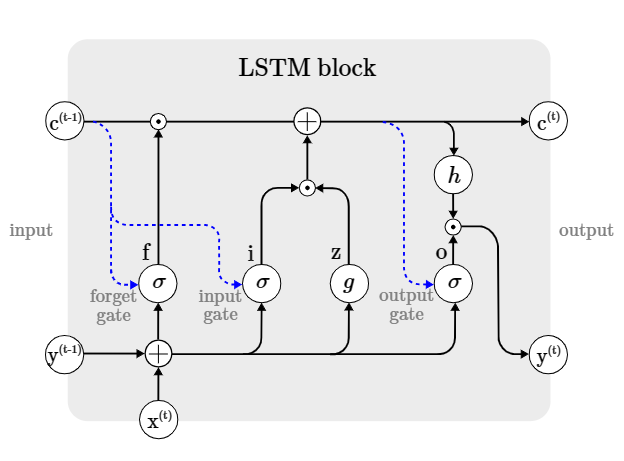
\includegraphics[width=0.31\textwidth]{LSTM.jpg}
	\caption{Architecture of the LSTM model.\centering}
	\label{fig1}
\end{figure}
The LSTM model is developed to address the long-term dependencies	problem of RNN. In RNNs, information can only propagate through a limited number of neurons, and the previous information tends to vanish as the models learn new information. The LSTM model attacks this problem by adding a forget gate, sorting out unnecessary information, enabling it to process only relevant data, and implying a better result. This is also the reason why the LSTM model is widely applied for time-series data prediction[15].\\
\indent To achieve such abilities, the LSTM put in use the cells and gates as follows:
\small
\begin{flalign*}
&\text{Forget gate (F):} & F_t &= \sigma(X_t W_{f} + h_{t-1} W_{f} + b_{f}) &\\
&\text{Input gate (I):} & I_t &= \sigma(X_t W_{i} + h_{t-1} W_{i} + b_{i}) &\\
&\text{Output gate (O):} & O_t &= \sigma(X_t W_{o} + h_{t-1} W_{o} + b_{o}) &\\
&\text{Candidate Memory Cell (C\_t):} & \tilde{C}_t &= \phi(X_t W_{c} + h_{t-1} W_{c} + b_{c}) &\\
&\text{Memory cell (C\_t):} & C_t &= F_t \odot C_{t-1} + I_t \odot \tilde{C}_t &\\
&\text{Hidden state (h):} & h_t &= \phi(c) \odot O_t &
\end{flalign*}
\noindent Where:
\begin{itemize}
  \item $X_t$: input at time $t$
  \item $F_t$: value at forget gate at time $t$
  \item $I_t$: value at input gate at time $t$
  \item $O_t$: value at output gate at time $t$
  \item $C_t$: is the memory cell at time $t$
  \item $h_t$: is the hidden state at time $t$
  \item $h_{t-1}$: is the hidden state from the previous layer
  \item $W_i, W_f, W_o, W_c$ are weight matrices
  \item $b_i, b_f, b_o, b_c$ are bias vectors
  \item $\odot$ is the Hadamard product
  \item $\sigma$ is the notation of the sigmoid activation function
  \item $\phi$ is the notation of the tanh activation function
\end{itemize}
\indent The forget gates are for sorting out necessary and unnecessary information. The input gate takes the current timestep $X_t$, the hidden state of the previous timestep, and determines where the information should be added to the long-term state. The output gate determines whether the output should be read. The candidate memory cell determines if the information passes to the cell state, and it uses tanh as the activation function. The memory cell allows LSTM to remember or forget the information, and the hidden state is the tool that enables the network to circulate information.
\subsection{Support Vector Regression}
Support vector regression (SVR) is a type of machine learning algorithm tries to find a function that best predicts the continuous output value for a given input value. SVR can use both linear and non-linear kernels, which are functions that determine the similarity between input vectors. The choice of kernel depends on the data’s characteristics and the task’s complexity[16].

\begin{table}[H]
\caption{Common kernel functions}
\renewcommand{\arraystretch}{2}
\centering
\begin{tabular}{|l|l|}
\hline
\textbf{Kernel} & \textbf{Function} \\ \hline
Polynomial kernel & $K(x, z) = (x^T z + b)$ \\ \hline
Radial basis (Gaussian) kernel & $K(x, z) = \exp\left(-\frac{\|x - z\|^2}{2\sigma^2}\right)$ \\ \hline
Exponential kernel & $K(x, z) = \exp\left(-\frac{\|x - z\|}{\sigma}\right)$ \\ \hline
\end{tabular}

\end{table}
\subsection{Extreme Gradient Boosting}
Extreme Gradient Boosting, is an advanced version of gradient boosting machines that is based on residual optimization. This algorithm aims for high efficiency, flexibility, and portability[]. XGBoost employs parallel boosting trees, establishing K regression trees to ensure the predicted values closely with the true values. With robust generalization capabilities, XGBoost can accurately address various scientific data challenges. Positioned as an enhanced algorithm of GBDT, its core lies in optimizing the objective function. The objective function of XGBoost can be expressed as[17]:
\[{obj}(\theta) = \sum_{i=1}^{n} l(y_i, \hat{y}) + \sum_{k=1}^{K} \Omega(f_k)\]
Where
\begin{itemize}
 \item \( l(y_i, \hat{y}) \): is the training error of the sample \(x_i\)
 \item \( \Omega(f_k) \):  represents the regular term of the first tree
 \item \(K\): represents the total number of trees, 
 \item \(f_k\): represents k the first tree
 \item \(f_k\): represents k the first tree
 \item \(\hat{y}\): represents the prediction result of the sample \(x_i\), and C is a constant


\end{itemize}
\subsection{Vector autoregression}
In the real world, there are a handful of cases where we can obtain groups of time series data presumably related to each other. In other words, we can predict their values not only by looking back on their historical data themselves but also by looking back at other variables’ lags. The fitting is symmetric with respect to variables. And, similarly to ARIMA, we can use differencing if the series are not stationary, and we can use the ADF test to make sure the data are ready for the regression.\\
Consider the case we have a group of three time series, denoted as y1,t, y2,t, y3,t and assume they are interrelated. The vector autoregression of order p or VAR(2) can be written as[14]:
\[
\begin{aligned}
y_{1,t} &= \phi_{01} + \phi_{11,1} X_{1,t-1} + \phi_{12,1} X_{2,t-1} + \phi_{13,1} X_{3,t-1} + \epsilon_{1,t} \\
&\quad + \phi_{11,2} X_{1,t-2} + \phi_{12,2} X_{2,t-2} + \phi_{13,2} X_{3,t-2} + \epsilon_{1,t-2} \\
y_{2,t} &= \phi_{02} + \phi_{21,1} X_{1,t-1} + \phi_{22,1} X_{2,t-1} + \phi_{23,1} X_{3,t-1} + \epsilon_{2,t} \\
&\quad + \phi_{21,2} X_{1,t-2} + \phi_{22,2} X_{2,t-2} + \phi_{23,2} X_{3,t-2} + \epsilon_{2,t-2} \\
y_{3,t} &= \phi_{03} + \phi_{31,1} X_{1,t-1} + \phi_{32,1} X_{2,t-1} + \phi_{33,1} X_{3,t-1} + \epsilon_{3,t} \\
&\quad + \phi_{31,2} X_{1,t-2} + \phi_{32,2} X_{2,t-2} + \phi_{33,2} X_{3,t-2} + \epsilon_{3,t-2}
\end{aligned}
\]

To generalize, their vector form of VAR(p) can be written as:
\[
y = \phi_0 + \phi_1 X_{t-1} + \phi_2 X_{t-2} + \ldots + \phi_p X_{t-p} + \epsilon
\]

Where:
\begin{itemize}
    \item \( y \): is the vector of variables at timestamp \( t \)
    \item \( \phi_0 \): is the \( 3 \times 1 \) matrix of intercepts
    \item \( \phi_i \): given that \( i \) is in \( [1, p] \), is the \( 3 \times 3 \) matrix of parameters
    \item \( y_{t-i} \): given that \( i \) is in \( [1, p] \), is the \( 3 \times 1 \) matrix of lags of variables
\end{itemize}

\subsection{Bi-LSTM}
The Bi-LSTM neural network is composed of LSTM units that operate in both directions to incorporate past and future context information. Bi-LSTM can learn long-term dependencies without retaining duplicate context information.[18]\\ 
Unlike the LSTM network, the Bi-LSTM network features two parallel layers that propagate in opposite directions with forward (left-to-right) and backward (right-to-left) passes to capture dependencies in two contexts.  Bi-directional LSTM predicts or tags the sequence of each element using a finite sequence based on the context of elements in the past and future.[19] In other words, by progressively processing the input in both directions, a Bi-directional LSTM can collect information from both past and future contexts, which is then combined and concatenated to produce the final output. As a result, it has shown great performance in sequential modeling issues and is commonly utilized in text classification. 
\begin{figure}[H]
	\centering
	\includegraphics[width=0.4\textwidth]{Bi-LSTM.png}
	\caption{Bi-LSTM visualization.\centering}
	\label{fig1}
\end{figure}

\subsection{CEEMDAN-LSTM}
When dealing with non-stationary, non-linear, and filled with outliers like financial time series, the participation of decomposition metrics that wipe out the uncertainties to spot the predictable patterns is crucial. In the paper “Financial time series forecasting model based on CEEMDAN and LSTM” (Jian Cao, Zhi Li, Jian Li. 2019), the combination of CEEMDAN and LSTM was first proposed.
\subsubsection{CEEMDAN}
CEEMDAN method is an adaptive signal time-frequency processing method that adds adaptive Gaussian white noise to the decomposition (Liang et al. 2019). This method is an improved version of EMD and EEMD that eventually eliminates the mixing mode, which causes similar oscillations in different modes, and the white noises remaining in the ensemble step[6][20]. \\
The CEEMDAN can be performed in the following steps:
\begin{itemize} 
    \item Adding different Gaussian white noise \( w^i(t) \) to the original series:
    \[ S^i(t) = S(t) + e_{0w}^i(t) \]
    
    \item Decompose the \( N \) new sequences by the EMD method and calculate the mean value to obtain the first modal component IMF\_1(t)
    \[ \text{mean}(\text{IMF}_1(t)) = \frac{1}{N} \sum_{i=1}^{N} \text{IMF}_1^i(t) \]
    
    \item Calculation of the first remaining component \( r_1(t) \)
    
    \item The signal is then decomposed using the EMD algorithm to gain the second modal component IMF\_2(t):
    \[ \text{IMF}_2(t) = \frac{1}{N} \sum_{i=1}^{N} E_1(r_1(t) + e_1 E_i(w^i(t))) \]
    
    \item Repeating steps (3) and (4) for \( k = 2,3,...,k \), so that we obtain:
    \begin{align*}
    r_k(t) &= r_{k-1}(t) - \text{IMF}_k(t) \\
    \text{IMF}_{k+1}(t) &= \frac{1}{N} \sum_{i=1}^{N} E_1(r_k(t) + e_k E_k(w^i(t)))
    \end{align*}
    
    \item The step (5) is repeated until the remaining components cannot be decomposed anymore, and finally, obtain a modal component. The final residuals of the decomposition are:
    \[ R(t) = S(t) - \sum_{i=1}^{K} \text{IMF}_i(t) \]
    The final original series is decomposed as:
    \[ S(t) = R(t) + \sum_{i=1}^{K} \text{IMF}_i(t) \]
\end{itemize}

\subsubsection{CEEMDAN - LSTM}
The combination of CEEMDAN and LSTM aims to decompose the series to IMFs, and then we apply the LSTM prediction to each IMF component and combine them to obtain the series of predicted values. The steps is performed like in the below flowchart:
\begin{figure}[H]
	\centering
	\includegraphics[width=0.4\textwidth]{CEEMDAN-LSTM.png}
	\caption{CEEMDAN-LSTM process\centering}
	\label{fig1}
\end{figure}
\subsection{Evaluation Metrics}
\subsubsection{RMSE}
While MSE can only measure the squared value for accuracy, the Root Mean Squared Error (RSME) can be measured in the same unit as the response variable. RMSE is the square root of the average squared error of the predicted Yi values:
\begin{align*}
    \text{RMSE} = \sqrt{\frac{\sum_{i=1}^{n} \big(\hat{y}_i - y_i\big)^2}{n}}
\end{align*}
This measures the model's overall accuracy and is a basis for comparing to other models. In other words, the smaller the RMSE gets, the more accurately our model can predict.

\subsubsection{MAPE}
Also related to error, the mean absolute percentage error (MAPE) is also a common measure to forecast errors. Apart from RSME, MAPE scales the error to percentage units, which assists our intuition in determining the efficiency of the model. However, MAPE is similar to RSE and RSME in terms of outliers, and this metric should work with non-zero data. This is the formula of MAPE:
\begin{align*}
    \text{MAPE} = \frac{1}{n} \sum_{t=1}^{n} \left| \frac{\hat{y}_i - y_i}{y_i} \right|
\end{align*}
Here, we can see that this formula, just like its name, gets the absolute percentage of variation of each predicted to the actual value, then sums them up and gets the mean of them.

\subsubsection{MAE}

The Mean Absolute Error (MAE) is the average of all absolute errors. The formula can be given as:

\[
\text{MAE} = \frac{1}{n} \sum_{i=1}^{n} \left| y_i - \hat{y}_i \right|
\]


\subsubsection{MSLE}
The use of Mean Squared Logarithmic Error(MSLE) is beneficial when dealing with predictions of values that span multiple orders of magnitude. MSLE penalizes underestimates and overestimates proportionally, taking into account the relative differences between predicted and actual values rather than absolute differences. The formula of MSLE is expressed as below:
\[\text{MSLE} = \frac{1}{n} \sum_{i=1}^{n} (\log(1 + y_i) - \log(1 + \hat{y}_i))^2
\]
Where:
\begin{itemize}
    \item $y_i$: the observed value.
    \item $\hat{y}_i$: the predicted value.
    \item $n$: the sample size of the dataset.
\end{itemize}


\section{Experiment}
\subsection{Data processing and description}

\subsubsection{SSI dataset}
\begin{figure}[H]
	\centering
	\includegraphics[width=0.5\textwidth]{SSI close price.png}
	\caption{SSI close price visualization.\centering}
	\label{fig1}
\end{figure}

\begin{figure}[H]
	\centering
	\includegraphics[width=0.5\textwidth]{SSI boxplot.png}
	\caption{SSI descriptive analysis.\centering}
	\label{fig1}
\end{figure}

\subsubsection{VND dataset}
\begin{figure}[H]
	\centering
	\includegraphics[width=0.5\textwidth]{VND  close price.png}
	\caption{VND close price visualization.\centering}
	\label{fig1}
\end{figure}

\begin{figure}[H]
	\centering
	\includegraphics[width=0.5\textwidth]{VND boxplot.png}
	\caption{VND descriptive analysis.\centering}
	\label{fig8}
\end{figure}

\subsubsection{VIB dataset}
\begin{figure}[H]
	\centering
	\includegraphics[width=0.5\textwidth]{VIB close price.png}
	\caption{VIB close price visualization.\centering}
	\label{fig1}
\end{figure}
\begin{figure}[H]
	\centering
	\includegraphics[width=0.5\textwidth]{VIB boxplot.png}
	\caption{VIB descriptive analysis.\centering}
	\label{fig1}
\end{figure}

\begin{table}[H]
\renewcommand{\arraystretch}{1.5}
\centering
\caption{Statistical Summary of 'Close' Column for Datasets SSI, VND, and VIB}
\label{tab:summary_statistics}
\begin{tabular}{lccc}

\rowcolor{headercolor}
\hline
\cellcolor{white} & \textbf{SSI} & \textbf{VND} &\textbf{VIB} \\ % Empty cell with white background
\hline
\cellcolor{firstcolcolor}Count & 1384.00 & 1385.00 & 1384.00 \\

\cellcolor{firstcolcolor}Mean & 13802.88 & 11775.59 & 13802.88 \\

\cellcolor{firstcolcolor}Std & 7741.37 & 9081.69 & 7741.37 \\

\cellcolor{firstcolcolor}Min & 4350.00 & 2530.00 & 4350.00 \\

\cellcolor{firstcolcolor}25\% & 5735.00 & 3650.00 & 5735.00 \\

\cellcolor{firstcolcolor}50\% & 14790.00 & 7270.00 & 14790.00 \\

\cellcolor{firstcolcolor}75\% & 20110.00 & 19300.00 & 20110.00 \\

\cellcolor{firstcolcolor}Max & 30520.00 & 34780.00 & 30520.00 \\

\cellcolor{firstcolcolor}Variance & 59928751.03 & 82477040.94 & 59928751.03 \\

\cellcolor{firstcolcolor}Std Dev & 7741.37 & 9081.69 & 7741.37 \\

\cellcolor{firstcolcolor}Range & 26170.00 & 32250.00 & 26170.00 \\

\cellcolor{firstcolcolor}IQR & 14375.00 & 15650.00 & 14375.00 \\

\cellcolor{firstcolcolor}Skewness & 0.22 & 0.68 & 0.22 \\

\cellcolor{firstcolcolor}Kurtosis & -1.36 & -0.79 & -1.36 \\
\hline
\end{tabular}
\end{table}

\subsection{Result}
Following the training and evaluation of the eight distinct machine learning and deep learning models as outlined earlier, employing three train-test split ratios (8:2, 7:3, and 6:4), we have selected the three most adept models for each dataset based on rigorous evaluation criteria. The ensuing predictions for the closing price in the subsequent 60 days for each stock, utilizing the chosen models, are delineated below:
\subsubsection{\textbf{SSI dataset}}
For SSI, both Support Vector Regression (SVR) and Vector Autoregressive (VAR) models demonstrate commendable performance, as evidenced by minimal errors in both testing phase.
\begin{figure}[H]
	\centering
	\includegraphics[width=0.5\textwidth]{SVR82_SSI.png}
	\caption{Predict SSI close price next 60 days using SVR (8:2 train-test ratio).\centering}
	\label{fig1}
\end{figure}

\begin{figure}[H]
	\centering
	\includegraphics[width=0.5\textwidth]{SVR73_SSI.png}
	\caption{Predict SSI close price next 60 days using SVR (7:3 train-test ratio).\centering}
	\label{fig1}
\end{figure}
\vspace*{-\baselineskip}
\begin{figure}[H]
	\centering
	\includegraphics[width=0.5\textwidth]{VAR82_SSI.png}
	\caption{Predict SSI close price next 60 days using VAR (8:2 train-test ratio).\centering}
	\label{fig1}
\end{figure}

\subsubsection{\textbf{VND dataset}}
In the case of VND, beside SVR and VAR, LSTM also showed a good performance
\begin{figure}[H]
	\centering
	\includegraphics[width=0.5\textwidth]{SVR82_VND.png}
	\caption{Predict VND close price next 60 days using SVR (8:2 train-test ratio).\centering}
	\label{fig1}
\end{figure}

\begin{figure}[H]
	\centering
	\includegraphics[width=0.5\textwidth]{VAR82_VND.png}
	\caption{Predict VND close price next 60 days using VAR (8:2 train-test ratio).\centering}
	\label{fig1}
\end{figure}

\begin{figure}[H]
	\centering
	\includegraphics[width=0.5\textwidth]{LSTM82_VND.png}
	\caption{Predict VND close price next 60 days using LSTM (8:2 train-test ratio).\centering}
	\label{fig1}
\end{figure}

\subsubsection{\textbf{VIB dataset}}
SVR and VAR also demonstrates good performance on this dataset
\begin{figure}[H]
	\centering
	\includegraphics[width=0.5\textwidth]{SVR82_VIB.png}
	\caption{Predict VIB close price next 60 days using SVR (8:2 train-test ratio).\centering}
	\label{fig1}
\end{figure}
\begin{figure}[H]
	\centering	\includegraphics[width=0.5\textwidth]{SVR73_VIB.png}
	\caption{Predict VIB close price next 60 days using SVR (7:3 train-test ratio).\centering}
	\label{fig1}
\end{figure}
\begin{figure}[H]
	\centering	\includegraphics[width=0.5\textwidth]{VAR82_VIB.png}
	\caption{Predict VIB close price next 60 days using VAR (8:2 train-test ratio).\centering}
	\label{fig1}
\end{figure}

\section{Evaluation}
Three statistical tables below demonstrate the result of evaluation of each model for each dataset using the four metrics specified above. Each table contains the model names along with the train-test ratio and the MAE, MRSE, MAPE, MSLE result determined based on the actual values and predicted values on the test set.

\noindent TABLE \ref{tab4} reveals the superior performance of SVR and VAR on the SSI dataset, as evidenced by significantly small figures across all four metrics with MAPE just around 2\% for both 8:2 and 7:3 ratios. In contrast, ARIMA and Linear Regression showcase inadequacy for this dataset, marked by notably large errors, up to 52\% of MAPE

\noindent In reviewing TABLE \ref{tab5}, it is evident that SVR and VAR continue to exhibit good performance for VND dataset. Conversely, LN, ARIMA, and CEEMDAN still display considerably large figures.

\noindent Looking at TABLE \ref{tab6} for VIB, beside SVR and VAR, LSTM and XGBoost demonstrate noteworthy results, with only slightly higher values in MAE and RMSE. Conversely, LN, ARIMA, and CEEMDAN still display considerably large figures.

\begin{table}[H]
\renewcommand{\arraystretch}{1.5}
\centering
\caption{Compare models' performance on SSI dataset}
\label{tab4}
\begin{tabular}{lp{1.1cm}p{1.2cm}p{1cm}p{0.9cm}}
\hline
\rowcolor{headercolor}
\textbf{MODEL}  & \textbf{MAE} & \textbf{RMSE} & \textbf{MAPE} & \textbf{MSLE}\\
\hline
\cellcolor{firstcolcolor} LN  8:2 & 5553.477 & 7430.082 & 20.608 & 0.142\\
\cellcolor{firstcolcolor} LN  7:3 & 6644.446 & 8272.427 & 25.526 & 0.095 \\
\cellcolor{firstcolcolor} LN  6:4 & 16068.788 & 18139.375 & 52.997 & 0.737\\
\cellcolor{firstcolcolor} ARIMA  8:2 & 5461.945 & 6094.900 & 24.497 & 0.068 \\
\cellcolor{firstcolcolor} ARIMA  7:3 & 9097.692 & 10331.529 & 46.071 & 0.173 \\
\cellcolor{firstcolcolor} ARIMA  6:4 & 8818.408 & 11353.932 & 27.199 & 0.167 \\
\cellcolor{firstcolcolor} SVR  8:2 & \textbf{504.422} & \textbf{695.531} & \textbf{2.226} & \textbf{0.001} \\
\cellcolor{firstcolcolor} SVR  7:3 & \textbf{596.739} & \textbf{814.360} & \textbf{2.403} & \textbf{0.001} \\
\cellcolor{firstcolcolor} SVR  6:4 & 10643.311 & 14983.691 & 30.848 & 0.096 \\
\cellcolor{firstcolcolor} LSTM  8:2 & 1444.358 & 1645.806 & 5.882 & 0.067 \\
\cellcolor{firstcolcolor} LSTM  7:3 & 1206.527 & 1480.558 & 4.578 & 0.054 \\
\cellcolor{firstcolcolor} LSTM  6:4 & 1960.211 & 2370.154 & 6.374 & 0.075 \\
\cellcolor{firstcolcolor} VAR  8:2 & \textbf{559.980} & \textbf{748.937} & \textbf{2.471} & \textbf{0.001} \\
\cellcolor{firstcolcolor} VAR  7:3 & \textbf{620.957} & \textbf{835.613} & 2.560 & \textbf{0.001} \\
\cellcolor{firstcolcolor} VAR  6:4 & 641.733 & 866.306 & \textbf{2.374} & \textbf{0.001} \\
\cellcolor{firstcolcolor} XGBoost  8:2 & 676.991 & 896.047 & 2.828 & \textbf{0.001} \\
\cellcolor{firstcolcolor} XGBoost  7:3 & 772.236 & 1008.766 & 3.059 & \textbf{0.001} \\
\cellcolor{firstcolcolor} XGBoost  6:4 & 7879.352 & 10757.625 & 22.831 & 0.141 \\
\cellcolor{firstcolcolor} Bi-LSTM  8:2 & 683.657 & 888.215 & 2.960 & 0.039 \\
\cellcolor{firstcolcolor} Bi-LSTM 7:3 & 856.901 & 1214.949 & 3.651 & 0.050 \\
\cellcolor{firstcolcolor} Bi-LSTM 6:4 & 885.792 & 1222.090 & 3.124 & 0.041 \\
\cellcolor{firstcolcolor} CEEMDAN-LSTM 8:2 & 7844.841 & 9494.712 & 24.923 & 0.132\\
\cellcolor{firstcolcolor} CEEMDAN-LSTM 7:3 & 8333.406 & 9756.357 & 26.407 & 0.135\\
\hline
\end{tabular}
\end{table}


\begin{table}[H]
\renewcommand{\arraystretch}{1.5}
\centering
\caption{Compare models' performance on VND dataset}
\label{tab5}
\begin{tabular}{lp{1.1cm}p{1.2cm}p{1cm}p{0.9cm}}
\hline
\rowcolor{headercolor}
\textbf{MODEL}  & \textbf{MAE} & \textbf{RMSE} & \textbf{MAPE} & \textbf{MSLE}\\
\hline
\cellcolor{firstcolcolor} LN 8:2 & 5845.904 & 6363.112 & 38.241 & 0.123\\
\cellcolor{firstcolcolor} LN 7:3 & 5292.054 & 7554.296 & 23.289 & 0.141\\
\cellcolor{firstcolcolor} LN 6:4 & 15540.490 & 16611.559 & 74.364 & 2.054\\
\cellcolor{firstcolcolor} ARIMA 8:2 & 5653.635 & 6365.051 & 37.871 & 0.126 \\
\cellcolor{firstcolcolor} ARIMA 7:3 & 12557.939 & 13723.772 & 75.599 & 0.352 \\
\cellcolor{firstcolcolor} ARIMA 6:4 & 10396.540 & 11445.631 & 55.586 & 0.266 \\
\cellcolor{firstcolcolor} SVR 8:2 & \textbf{433.137} & \textbf{575.545} & \textbf{2.593} & \textbf{0.001} \\
\cellcolor{firstcolcolor} SVR 7:3 & 614.076 & 907.944 & \textbf{3.073} & 0.002 \\
\cellcolor{firstcolcolor} SVR 6:4 & 14190.093 & 15419.864 & 66.749 & 1.445 \\
\cellcolor{firstcolcolor} LSTM 8:2 & \textbf{542.273} & \textbf{717.212} & 3.343 & 0.045 \\
\cellcolor{firstcolcolor} LSTM 7:3 & 830.321 & 1237.961 & 4.006 & 0.054 \\
\cellcolor{firstcolcolor} LSTM 6:4 & 1026.057 & 1391.083 & 4.502 & 0.057 \\
\cellcolor{firstcolcolor} VAR 8:2 & \textbf{483.932} & \textbf{628.544} & \textbf{2.873} & \textbf{0.001} \\
\cellcolor{firstcolcolor} VAR 7:3 & 672.511 & 884.690 & 3.541 & 0.002 \\
\cellcolor{firstcolcolor} VAR 6:4 & 579.551 & 758.981 & \textbf{2.947} & \textbf{0.001} \\
\cellcolor{firstcolcolor} XGBoost 8:2 & \textbf{536.848} & \textbf{672.888} & 3.219 & 0.002 \\
\cellcolor{firstcolcolor} XGBoost 7:3 & 734.119 & 929.698 & 3.735 & 0.002 \\
\cellcolor{firstcolcolor} XGBoost 6:4 & 10280.315 & 11813.687 & 46.387 & 0.520 \\
\cellcolor{firstcolcolor} Bi-LSTM 8:2 & 1032.117 & 1368.804 & 6.933 & 0.094 \\
\cellcolor{firstcolcolor} Bi-LSTM 7:3 & 1619.118 & 2606.460 & 7.223 & 0.106 \\
\cellcolor{firstcolcolor} Bi-LSTM 6:4 & 648.202 & 867.141 & 3.190 & 0.042 \\
\cellcolor{firstcolcolor} CEEMDAN-LSTM 8:2 & 3555.426 & 4424.971 & 20.076 & 0.077\\
\cellcolor{firstcolcolor} CEEMDAN-LSTM 7:3 & 3445.275 & 4118.283 & 16.564 & 0.084\\
\cellcolor{firstcolcolor} CEEMDAN-LSTM 6:4 & 4211.870 & 4783.066 & 20.208 & 0.083\\
\hline

\end{tabular}
\end{table}
\begin{table}[h]
\renewcommand{\arraystretch}{1.5}
\centering
\caption{Compare models' performance on VIB dataset}
\label{tab6}
\begin{tabular}{lp{1.1cm}p{1.2cm}p{1cm}p{0.9cm}}
\hline
\rowcolor{headercolor}
\textbf{MODEL}  & \textbf{MAE} & \textbf{RMSE} & \textbf{MAPE} & \textbf{MSLE}\\
\hline
\cellcolor{firstcolcolor} LN 8:2 & 7901.845 & 8020.619 & 44.993 & 0.142\\
\cellcolor{firstcolcolor} LN 7:3 & 5913.124 & 6330.068 & 31.713 & 5913.124\\
\cellcolor{firstcolcolor} LN 6:4 & 5948.984 & 7880.072 & 25.466 & 0.184\\
\cellcolor{firstcolcolor} ARIMA 8:2 & 2063.110 & 2581.220 & 12.552 & 0.021 \\
\cellcolor{firstcolcolor} ARIMA 7:3 & 10936.211 & 12038.006 & 61.084 & 0.253 \\
\cellcolor{firstcolcolor} ARIMA 6:4 & 3169.926 & 4220.816 & 14.425 & 0.042 \\
\cellcolor{firstcolcolor} SVR 8:2 & \textbf{252.801} & \textbf{346.719} & \textbf{1.453} & \textbf{0.000} \\
\cellcolor{firstcolcolor} SVR 7:3 & \textbf{318.958} & 444.228 & \textbf{1.657} & \textbf{0.001} \\
\cellcolor{firstcolcolor} SVR 6:4 & 2325.337 & 4647.332 & 8.984 & 0.048 \\
\cellcolor{firstcolcolor} LSTM 8:2 & 336.270 & 462.350 & 1.955 & 0.028 \\
\cellcolor{firstcolcolor} LSTM 7:3 & 495.757 & 676.101 & 2.721 & 0.037 \\
\cellcolor{firstcolcolor} LSTM 6:4 & 3070.414 & 3364.997 & 14.429 & 0.164 \\
\cellcolor{firstcolcolor} VAR 8:2 & 372.819 & 506.260 & 1.816 & 0.001 \\
\cellcolor{firstcolcolor} VAR 7:3 & \textbf{322.668} & \textbf{437.685} & \textbf{1.687} & \textbf{0.001} \\
\cellcolor{firstcolcolor} VAR 6:4 & 266.311 & \textbf{352.757} & \textbf{1.517} & \textbf{0.000} \\
\cellcolor{firstcolcolor} XGBoost 8:2 & \textbf{316.219} & \textbf{414.142} & 1.821 & 0.001 \\
\cellcolor{firstcolcolor} XGBoost 7:3 & 424.014 & 566.261 & 2.219 & 0.001 \\
\cellcolor{firstcolcolor} XGBoost 6:4 & 762.678 & 1153.545 & 3.480 & 0.002 \\
\cellcolor{firstcolcolor} Bi-LSTM 8:2 & 425.319 & 579.586 & 2.501 & 0.035 \\
\cellcolor{firstcolcolor} Bi-LSTM 7:3 & 1024.614 & 1329.638 & 5.530 & 0.069 \\
\cellcolor{firstcolcolor} Bi-LSTM 6:4 & 1030.012 & 1533.446 & 4.621 & 0.066 \\
\cellcolor{firstcolcolor} CEEMDAN-LSTM 8:2 & 1891.163 & 2347.289& 10.446& 0.017\\
\cellcolor{firstcolcolor} CEEMDAN-LSTM 7:3 & 2322.955 & 3011.204 & 12.204 & 0.053\\
\cellcolor{firstcolcolor} CEEMDAN-LSTM 6:4 & 7160.189 & 8144.200 & 32.558 & 0.203 \\
\hline
\end{tabular}
\end{table}

\section{Discussion and Conclusion}
In this article, we have performed and compared eight machine learning and deep learning models in financial series analysis and forecasting. We chose three datasets with similar behaviors from VietstockFinance as the target and used MAE, RSME, MAPE, MSLE to evaluate their accuracy. From the result, we can see that VAR and SVR gave the best modeling. And LSTM, Bi-LSTM, XGBoost also gave a good performance. On the other hand, Linear Regression and ARIMA, whose advantages are the simplicity had relatively high MAPE, MAE, and RSME, which means their forecast results may not be reliable. Finally, the combination of CEEMDAN and LSTM, which aims to decompose the signal into smaller components, and then train LSTM models with each component, did not work well, as they only gave a decent forecasting result, even worse than the original LSTM. 

\section{Future Orientations}
As for some issues with the CEEMDAN-LSTM model, in the future, we plan to optimize the CEEMDAN decomposed signal processing, reduce the complexity and loss during the transformation of the data, and tune the hyperparameters of the LSTM model. Hopefully, we can improve the overall prediction accuracy of the method. Additionally, as for the result, we found that the proposed models may not be the best fit for the data we are working with, so we will take some time to find some other combinations and processing methods that can deal with such highly volatile data as the one we obtained. Finally, the stock data is just a part of a bigger picture, as it only reflects how the market thinks of a company as a whole. However, the forecast result, methods, and processes can be developed into parts of other studies about business evaluation, or risk management applications. 

\section{References}

[1] Brown, S. J., Goetzmann, W. N., \& Kumar, A. (1998b). The Dow Theory: William Peter Hamilton’s track record reconsidered. The Journal of Finance, 53(4), 1311–1333. 

\noindent[2] Lee, C., \& Ko, C. (2011). Short-term load forecasting using lifting scheme and ARIMA models. Expert Systems With Applications, 38(5), 5902–5911.

\noindent[3] Bauer, P., Thorpe, A., \& Brunet, G. (2015). The quiet revolution of numerical weather prediction. Nature, 525(7567), 47–55.

\noindent[4] Fan, J., Wang, X., Wu, L., Zhou, H., Zhang, F., Lu, X., \& Xiang, Y. (2018). Comparison of Support Vector Machine and Extreme Gradient Boosting for predicting daily global solar radiation using temperature and precipitation in humid subtropical climates: A case study in China. Energy Conversion and Management, 164, 102–111. 

\noindent[5] Shahid, F., Zameer, A., \& Muneeb, M. (2020). Predictions for COVID-19 with deep learning models of LSTM, GRU and Bi-LSTM. Chaos, Solitons \& Fractals, 140, 110212. 

\noindent[6] Cao, J., Li, B., \& Li, J. (2019). Financial time series forecasting model based on CEEMDAN and LSTM. Physica A: Statistical Mechanics and Its Applications, 519, 127–139.

\noindent[7] Pramod, \& Pm, M. S. (2021). Stock Price Prediction Using LSTM

\noindent[8] Cao, J., Li, B., \& Li, J. (2019). Financial Time Series Forecasting Model Based on CEEMDAN and LSTM.

\noindent[9] Vuong, P. H., Trinh, T. D., Khoi, T., \& Uyen, P. H. (2022). Stock-Price Forecasting Based on XGBOOST and LSTM.

\noindent[10] Ma, Q. (2020). Comparison of ARIMA, ANN, and LSTM for Stock Price Prediction.

\noindent[11] Hao, W., \& Yu, S. (2006). Support Vector Regression for Financial Time Series Forecasting.

\noindent[12] Lemya, T.A. (2021). Forecasting Time Series Using Vector Autoregressive Model.

\noindent[13] Peter Bruce, Andrew Bruce \& Peter Gedeck (2017). Practical Statistics for Data Scientists (Second Edition)

\noindent[14] Aileen Nielsen (2019). Practical Time Series Analysis

\noindent[15] Hochreiter, S., \& Schmidhuber, J. (1997). Long Short-Term memory. Neural Computation, 9(8), 1735–1780.

\noindent[16]Balabin, R. M., \& Lomakina, E. I. (2011). Support vector machine regression (SVR/LS-SVM)—an alternative to neural networks (ANN) for analytical chemistry? Comparison of nonlinear methods on near infrared (NIR) spectroscopy data. Analyst, 136(8), 1703. 

\noindent[17] Luo, J., Zhang, Z., Fu, Y., \& Rao, F. (2021). Time series prediction of COVID-19 transmission in America using LSTM and XGBoost algorithms. Results in Physics, 27, 104462. 

\noindent [18] Jang, B., Kim, M., Harerimana, G., Kang, S. U., \& Kim, J. W. (2020). Bi-LSTM model to increase accuracy in text classification: combining Word2VEC CNN and Attention Mechanism. Applied Sciences, 10(17), 5841. 

\noindent [19]Hamayel, M. J., \& Owda, A. Y. (2021b). A novel cryptocurrency price prediction model using GRU, LSTM and bi-LSTM machine learning algorithms. AI, 2(4), 477–496. 

\noindent[20]Cao, J., Li, B., & Li, J. (2019b). Financial time series forecasting model based on CEEMDAN and LSTM. Physica A: Statistical Mechanics and Its Applications, 519, 127–139. 
\EOD
\end{document}
